\documentclass[letterpaper, 11pt]{extarticle}
% \usepackage{fontspec}

% ==================================================

% document parameters
% \usepackage[spanish, mexico, es-lcroman]{babel}
\usepackage[english]{babel}
\usepackage[margin = 1in]{geometry}

% ==================================================

% Packages for math
\usepackage{mathrsfs}
\usepackage{amsfonts}
\usepackage{amsmath}
\usepackage{amsthm}
\usepackage{amssymb}
\usepackage{physics}
\usepackage{dsfont}
\usepackage{esint}

% ==================================================

% Packages for writing
\usepackage{enumerate}
\usepackage[shortlabels]{enumitem}
\usepackage{framed}
\usepackage{csquotes}

% ==================================================

% Miscellaneous packages
\usepackage{float}
\usepackage{tabularx}
\usepackage{xcolor}
\usepackage{multicol}
\usepackage{subcaption}
\usepackage{caption}
\usepackage{appendix}
\captionsetup{format = hang, margin = 10pt, font = small, labelfont = bf}

% Citation
\usepackage[round, authoryear]{natbib}

% Hyperlinks setup
\usepackage{hyperref}
\definecolor{links}{rgb}{0.36,0.54,0.66}
\hypersetup{
   colorlinks = true,
    linkcolor = black,
     urlcolor = blue,
    citecolor = blue,
    filecolor = blue,
    pdfauthor = {Author},
     pdftitle = {Title},
   pdfsubject = {subject},
  pdfkeywords = {one, two},
  pdfproducer = {LaTeX},
   pdfcreator = {pdfLaTeX},
   }
\usepackage{titlesec}
\usepackage[many]{tcolorbox}

% Adjust spacing after the chapter title
\titlespacing*{\chapter}{0cm}{-2.0cm}{0.50cm}
\titlespacing*{\section}{0cm}{0.50cm}{0.25cm}

% Indent 
\setlength{\parindent}{0pt}
\setlength{\parskip}{1ex}

% --- Theorems, lemma, corollary, postulate, definition ---
% \numberwithin{equation}{section}

\newtcbtheorem[]{problem}{Problem}%
    {enhanced,
    colback = black!5, %white,
    colbacktitle = black!5,
    coltitle = black,
    boxrule = 0pt,
    frame hidden,
    borderline west = {0.5mm}{0.0mm}{black},
    fonttitle = \bfseries\sffamily,
    breakable,
    before skip = 3ex,
    after skip = 3ex
}{problem}

\tcbuselibrary{skins, breakable}

% --- You can define your own color box. Just copy the previous \newtcbtheorm definition and use the colors of yout liking and the title you want to use.
% --- Basic commands ---
%   Euler's constant
\newcommand{\eu}{\mathrm{e}}

%   Imaginary unit
\newcommand{\im}{\mathrm{i}}

%   Sexagesimal degree symbol
\newcommand{\grado}{\,^{\circ}}

% --- Comandos para álgebra lineal ---
% Matrix transpose
\newcommand{\transpose}[1]{{#1}^{\mathsf{T}}}

%%% Comandos para cálculo
%   Definite integral from -\infty to +\infty
\newcommand{\Int}{\int\limits_{-\infty}^{\infty}}

%   Indefinite integral
\newcommand{\rint}[2]{\int{#1}\dd{#2}}

%  Definite integral
\newcommand{\Rint}[4]{\int\limits_{#1}^{#2}{#3}\dd{#4}}

%   Dot product symbol (use the command \bigcdot)
\makeatletter
\newcommand*\bigcdot{\mathpalette\bigcdot@{.5}}
\newcommand*\bigcdot@[2]{\mathbin{\vcenter{\hbox{\scalebox{#2}{$\m@th#1\bullet$}}}}}
\makeatother

%   Hamiltonian
\newcommand{\Ham}{\hat{\mathcal{H}}}

%   Trace
\renewcommand{\Tr}{\mathrm{Tr}}

% Christoffel symbol of the second kind
\newcommand{\christoffelsecond}[4]{\dfrac{1}{2}g^{#3 #4}(\partial_{#1} g_{#2 #4} + \partial_{#2} g_{#1 #4} - \partial_{#4} g_{#1 #2})}

% Riemann curvature tensor
\newcommand{\riemanncurvature}[5]{\partial_{#3} \Gamma_{#4 #2}^{#1} - \partial_{#4} \Gamma_{#3 #2}^{#1} + \Gamma_{#3 #5}^{#1} \Gamma_{#4 #2}^{#5} - \Gamma_{#4 #5}^{#1} \Gamma_{#3 #2}^{#5}}

% Covariant Riemann curvature tensor
\newcommand{\covariantriemanncurvature}[5]{g_{#1 #5} R^{#5}{}_{#2 #3 #4}}

% Ricci tensor
\newcommand{\riccitensor}[5]{g_{#1 #5} R^{#5}{}_{#2 #3 #4}}

\begin{document}

\begin{Large}
    \textsf{\textbf{Stochastic Linear Bandits}}
    An Empirical Study
\end{Large}

\vspace{1ex}

\textsf{\textbf{Students:}} \text{Antani Gospodinov, Martin Jolif}, \\
\textsf{\textbf{Lecturer:}} \text{Claire Vernade}, Find my email on my \href{www.cvernade.com}{website}
\vspace{2ex}

\section{Linear Epsilon Greedy}
\subsection{Implementation of Linear Bandit environment and action generation function}
To implement the action generation function we will use fact that if $ X = (X_1, X_2, \ldots, X_n) \sim \mathcal{N}(0, I_n) $, 
then $ Y = X / \sqrt{X_1^2 + \ldots + X_n^2} $ is uniformly distributed on the surface of the unit sphere. It is an immediate
consequence that for $Y$ as defined above and $\mu \in \mathbb{R}^n$, $ Y + \mu$ is uniformly distributed on a sphere with unit radius,
centered at the point $\mu$. With that in mind, we propose the following implementation for the aciton generation function:
\begin{verbatim}
def ActionsGenerator(K,d,mean=None):
  res = np.random.normal(0,1,size=(K, d))
  norms = np.linalg.norm(res,axis=1)
  res /= norms[:,np.newaxis]
  if mean is not None:
    res += mean
  return res
\end{verbatim}
Implementation of the \textbf{LinearBandit} environment is straightforward and can be seen in the appendix.
\subsection{Implementation and Benchmark of Linear Epsilon Greedy}
We follow the equations given on p. 242 in \cite{lattimore2020bandit} to update our confidence ellipsoid for $\theta$
and to compute $\hat{\theta}$ at every time step. We try the algorithm on two environments: both of them have $K=50$ and $d=10$,
but one of them has a fixed action set and the other doesn't. We plot the regrets achieved by agents using different values of $\epsilon$.
In the fixed action set environment we observe a clear bias-variance tradeoff between the chosen values for $\epsilon$. 
Interestingly(\emph{but perhaps not surprisingly}), the results look quite different in the environment with a changing action set. A bias-variance
tradeoff can still be observed, but it is significantly less pronounced. To provide a plausible explanation we also plot the spectral norms for the
confidence ellipsoid matrices over time, with the idea being that the largest singular value $\sigma_1$ bounds the distance between $\hat{\theta}$
and $\theta$. It turns out that the graphs of spectral norms are mostly equivalent between different values for $\epsilon$ - and this makes a lot of sense, 
because with an ever-changing action set we gain the benefits of exploration for free! The small difference in variance can be explained by the fact that
in the exploitation steps we choose the most collinear to $\theta$ action, but to maximize the obtained information about $\theta$ we should choose the most
orthogonal action to the span of all actions we've chosen so far - and these two choices are conflicting. You can find the results of the experiment in the
appendix.

\subsection{Performance analysis of different matrix inversion methods for updating the confidence ellipsoid}
We compare three different methods for updating the confidence ellipsoid matrix between timesteps:
\begin{itemize}
  \item classic matrix inversion via \textbf{numpy.linalg.inv} - $\mathcal{O}(d^3)$ time complexity
  \item approximate matrix inversion via \textbf{numpy.linalg.lstsq} - $\mathcal{O}(d^3)$ time complexity
  \item Sherman-Morrison formula for computing the inverse of a matrix after rank-1 update - $\mathcal{O}(d^2)$ time complexity
\end{itemize}
We use two benchmarks to compare the methods. In the first one we observe the runtimes of agents in a number of environments
with a fixed \textit{arm-dimension} $d$ and a varying number of arms $K$. In the second benchmark we switch things up and instead fix $d$
and let $K$ vary. The experiments confirm our intuition that the method based on the Sherman-Morrison formula has the best performance as the
arm-dimension $d$ increases.

\begin{figure}[h!]
  \centering
  % First plot
  \begin{subfigure}[b]{0.45\textwidth}
      \centering
      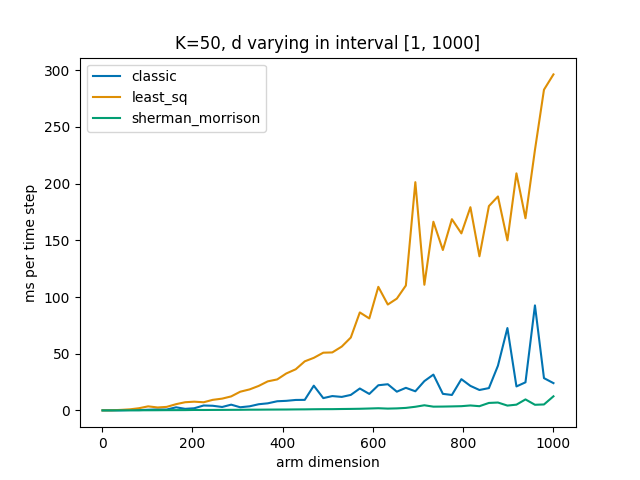
\includegraphics[width=\textwidth]{plots/d_varying_time.png}
      \label{fig:plot1}
  \end{subfigure}
  \hfill
  % Second plot
  \begin{subfigure}[b]{0.45\textwidth}
      \centering
      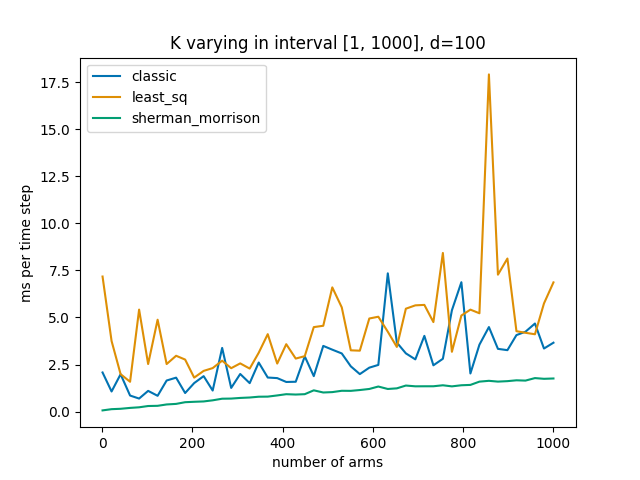
\includegraphics[width=\textwidth]{plots/K_varying_time.png}
      \label{fig:plot2}
  \end{subfigure}
  \label{fig:combined_plots}
  \caption{Performance analysis of different matrix inversion schemes}
\end{figure}

\section{Problem 2}

\subsection{Implementation of \textbf{LinUCB} and \textbf{LinTS}}
For the implementation of LinUCB, we are choosing the next arm with the following formula where the first term is an exploitation term and 
second one is an exploration bonus:
\[ A_{t+1} = argmax_{a \in \mathbb{A}} a^T \hat \theta_t^{\lambda} + {\lVert a \rVert}_{{(B_t^{\lambda})}^{-1}} \beta(t,\delta) \]
This corresponds to choose the next arm with the highest Upper Confidence Bound.

For the implementation of LinTS, we are drawing a possible sample from the posterior distribution before acting optimally in this sampled model:
\[ \tilde{\theta}_t \sim \mathcal{N}(\hat \theta_t^{\lambda}, 
   \sigma^2{(B_t^{\lambda})}^{-1}) \text{ and, } A_{t+1} = argmax_{a \in \mathbb{A}} a^T \tilde{\theta}_t\]


\newgeometry{top=0.7cm}
\subsection{Thompson sampling posterior at time \emph{t}}
We have $\mathbb{P}_{prior}(\theta_{\star}) \sim \mathcal{N}(\mathbf{0}, \lambda \mathbf{I}_d)$ and we assume that for all $t$, $Y_{t} = \theta_{\star}^TA_t + \epsilon_t$ and $\epsilon_t \sim \mathcal{N}(0, \sigma^2)$.

We will reason by induction and suppose that the posterior distribution follows:

\[
\theta_{\star}|A_1, Y_1, \dots, A_t, Y_t \sim \mathcal{N}(\hat\theta_t^{\lambda}, \sigma^2{(B_t^{\lambda})}^{-1})
\]

where $B_t^{\lambda} = \lambda \mathbf{I}_d + \sum_{s=1}^t A_s A_s^T$ and $\hat\theta_t^{\lambda} = {(B_t^{\lambda})}^{-1} (\sum_{s=1}^t Y_s A_s)$

\medskip
We suppose the statement is true at time step $t$ and we want to show it holds at time step $t+1$:
\begin{align*}
    \mathbb{P}_{\text{post}}^{t+1}(\theta_{\star}) & \propto \mathcal{L}(\theta_{\star} | A_1, Y_1, \dots A_t, Y_t, A_{t+1}, Y_{t+1}) \mathbb{P}_{prior}(\theta_{\star})\\
    & \propto \mathbb{P}(A_{t+1}, Y_{t+1} | \theta_{\star}) \mathcal{L}(\theta_{\star} | A_1, Y_1, \dots A_t, Y_t) \mathbb{P}_{prior}(\theta_{\star}) \\
    & \propto \mathbb{P}(A_{t+1}, Y_{t+1} | \theta_{\star}) \mathbb{P}_{\text{post}}^{t}(\theta_{\star}) \\
    & \propto e^{-\frac{1}{2\sigma^2} (Y_{t+1} - \theta_{\star}^TA_{t+1})^2} e^{-\frac{1}{2\sigma^2}(\theta_{\star} - \hat\theta_t^{\lambda})^T B_t^{\lambda}(\theta_{\star} - \hat\theta_t^{\lambda}) }\\
    & \propto e^{-\frac{1}{2\sigma^2}(Y_{t+1}^2 -2\theta_{\star}^TA_{t+1}Y_{t+1} + \theta_{\star}^TA_{t+1}A_{t+1}^T\theta_{\star} + \theta_{\star}^T B_t^{\lambda}\theta_{\star} - 2\theta_{\star}^T B_t^{\lambda}\hat\theta_t^{\lambda})}\\
    & \propto e^{-\frac{1}{2\sigma^2}(\theta_{\star}^T (B_t^{\lambda} + A_{t+1}A_{t+1}^T) \theta_{\star} -2 \theta_{\star}^T (B_t^{\lambda} + A_{t+1}A_{t+1}^T) (\hat\theta_{t}^{\lambda} + Y_{t+1}A_{t+1})  )} = e^{-\frac{1}{2\sigma^2}(\theta_{\star}^T B_{t+1}^{\lambda}  \theta_{\star} -2 \theta_{\star}^T B_{t+1}^{\lambda} \hat\theta_{t+1}^{\lambda})}\\
    & \propto e^{-\frac{1}{2\sigma^2}{(\theta_{\star} - \hat\theta_{t+1}^{\lambda})}^T B_{t+1}^{\lambda}  (\theta_{\star} - \hat\theta_{t+1}^{\lambda})}
\end{align*}

Therefore:
$\theta_{\star}|A_1, Y_1, \dots, A_{t+1}, Y_{t+1} \sim \mathcal{N}(\hat\theta_{t+1}^{\lambda}, \sigma^2{(B_{t+1}^{\lambda})}^{-1})$

\subsection{Comparing different algorithms}
Now, we want to compare the different algorithms proposed before and try to figure out which one could be the best.
To do so, we set our environment to be the classical Linear Bandit environment, we choose the following parameters $K=7, N=50$ (number of Monte Carlo Simulations), $\delta = \frac{1}{T}$ and $\sigma = 1$.

\begin{figure}[h]
      \centering
      \begin{subfigure}[b]{0.48\textwidth}
          \centering
          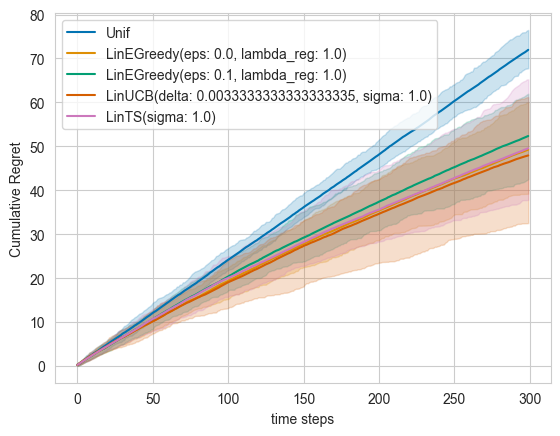
\includegraphics[width=\textwidth]{plots/output.png}
          \caption{Arm dimension (d=32)}
      \end{subfigure}
      \hfill
      \begin{subfigure}[b]{0.48\textwidth}
          \centering
          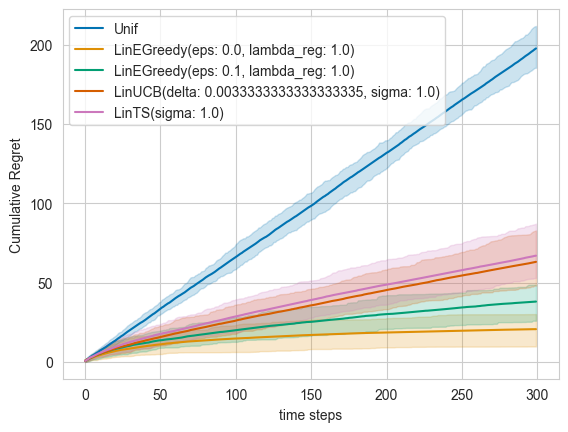
\includegraphics[width=\textwidth]{plots/output1.png}
          \caption{Arm dimension (d=4)}
      \end{subfigure}
\end{figure}

Clearly the uniform choice is not the best one as expected, however, for the other algorithm, it's more difficult to say if there is a best one. 
Indeed, it depends on a lot of different parameters like the arm dimension, the number of arms, or the parameters $\delta$ or $\lambda$.
Each algorithm can be better with specific hypothesis.



% =================================================

% \newpage

% \vfill
%%% Reminder: Maximum 3 pages
\newpage

\bibliographystyle{apalike}
\bibliography{references}


\appendix

\section{Bonus section: The role of the action set}

This last part allows you to study how certain actions sets can be hard for LinUCB. I propose some code to highlight this phenomenon, that was unveiled by \citet{lattimore2017end}. 
Follow the instructions in the notebook and report your results and comments here. 
\emph{This part can count up to (+2) points, meaning that the maximal grade is (12/10) and could compensate missed points on the Quiz or on the project. }

\section{Benchmark of \textbf{Linear Epsilon Greedy}}
\begin{figure}[H]
  \centering
  % Top-left plot
  \begin{subfigure}{0.45\textwidth}
      \centering
      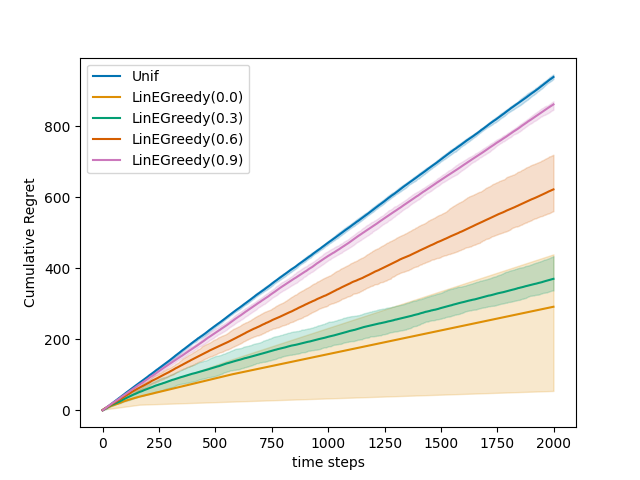
\includegraphics[width=\linewidth]{plots/regret_e_greedy_fixed_actions.png}
  \end{subfigure}
  % Top-right plot
  \begin{subfigure}{0.45\textwidth}
      \centering
      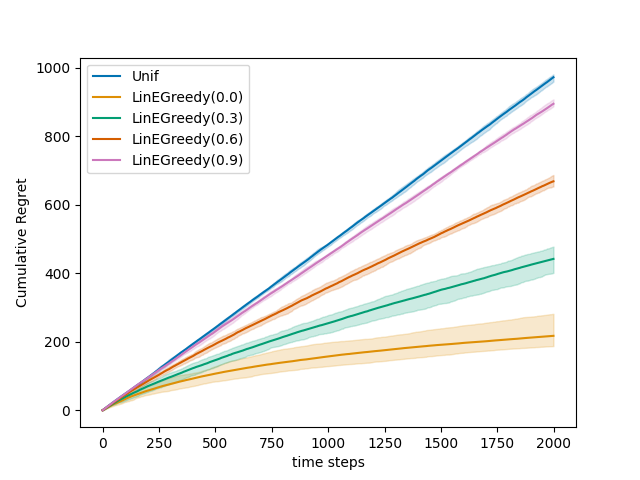
\includegraphics[width=\linewidth]{plots/regret_e_greedy_varying_actions.png}
  \end{subfigure}
  % Bottom-left plot
  \begin{subfigure}{0.45\textwidth}
      \centering
      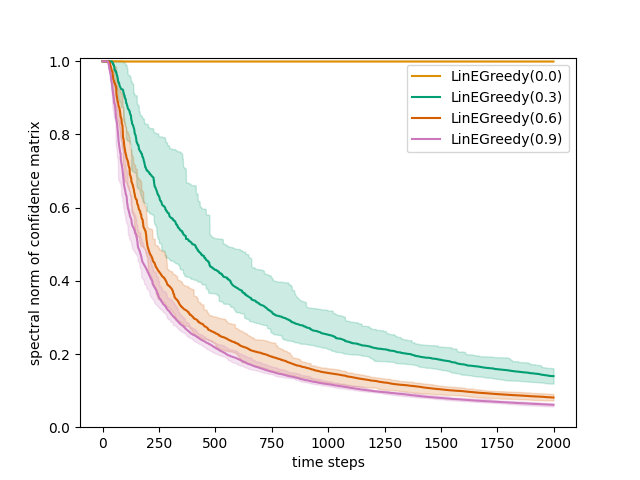
\includegraphics[width=\linewidth]{plots/spectral_norms_e_greedy.png}
      \caption{Fixed action set}
  \end{subfigure}
  % Bottom-right plot
  \begin{subfigure}{0.45\textwidth}
      \centering
      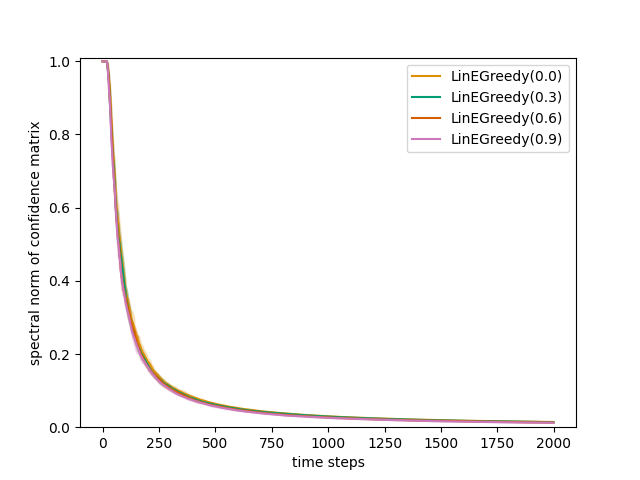
\includegraphics[width=\linewidth]{plots/spectral_norms_e_greedy_varying_actions.png}
      \caption{Changing action set}
  \end{subfigure}

  \caption{Benchmark on \textbf{Linear Epsilon Greedy}}
  \label{fig:2x2_plots}
\end{figure}


\section{Implementation of \textbf{Linear Bandit} environment}
\begin{verbatim}
class LinearBandit:
def __init__(self, theta, K, var=1., fixed_actions=None):
  """
  theta: d-dimensional vector (bounded) representing the hidden parameter
  K: number of actions per round (random action vectors generated each time)
  pb_type: string in 'fixed', 'iid', 'nsr' (please ignore NotSoRandom)
  """
  self.d = np.size(theta)
  self.theta = theta
  self.K = K
  self.var = var
  self.fixed_actions = fixed_actions
  self.current_action_set = self.get_action_set()

def get_action_set(self):
  """
  Generates a set of vectors in dimension self.d. Use your ActionsGenerator
  Alternatively, the set of actions is fixed a priori (given as input).
  Implement a condition to return the fixed set when one is given
  """
  if self.fixed_actions is not None:
    return self.fixed_actions
  else:
    self.current_action_set = ActionsGenerator(self.K, self.d)
    return self.current_action_set

def get_reward(self, action):
  """ sample reward given action and the model of this bandit environment
  action: d-dimensional vector (action chosen by the learner)
  """
  mean = np.dot(action, self.theta)
  return np.random.normal(mean, scale=self.var)

def get_means(self):
  return np.dot(self.current_action_set, self.theta)
\end{verbatim}


\section{Implementation of LinUCB and LinTS}

\begin{verbatim}
def get_action(self, arms):
  K, _ = arms.shape
  #compute np.sqrt(x.T @ A @ x) for each row x of the matrix arms
  norm_arms = np.sqrt(np.einsum('ij,jk,ik->i', arms, self.invcov, arms))
  L = 1
  beta = self.sigma * np.sqrt(2*np.log(1/self.delta) \+ 
    self.d*np.log(1+self.t*(L/(self.d*self.lambda_reg)))) \+
    np.sqrt(self.lambda_reg)
  UCB = arms @ self.hat_theta + norm_arms*beta
  return arms[np.argmax(UCB)]
\end{verbatim}
\begin{verbatim}
def get_action(self, arms):
  K, _ = arms.shape
  X = np.random.normal(0, 1, self.d)
  tilde_theta = self.hat_theta + self.sigma * np.linalg.cholesky(self.invcov) @ X
  return arms[np.argmax(arms @ tilde_theta)]
\end{verbatim}


\end{document}